%% This is emulateapj reformatting of the AASTEX sample document
%%

% Does not compile using BibTex
\documentclass{emulateapj}

\errorcontextlines 10000

\usepackage{cleveref}
\usepackage{amsmath}

\renewcommand*{\thefootnote}{\fnsymbol{footnote}}

%\renewcommand{\baselinestretch}{1.3}

\slugcomment{\today} % Ich glaube das ist "doppelt gemoppelt"; nur submitted reicht
\submitted{\newline\today}

\bibliographystyle{abbrvnat}
\setcitestyle{super, open={(}, end={)}}

\makeatletter
\newcommand\footnoteref[1]{\protected@xdef\@thefnmark{\ref{#1}}\@footnotemark}
\makeatother

\makeatletter % @ as normal letter symbol
\long\def\frontmatter@title@above{} % remove unwanted stuff in header
\newcommand\plotthree[3]{ % define command for three plots in a row
  \centering
  \leavevmode
  \setlength{\plot@width}{0.3\linewidth}
  \includegraphics[width={\eps@scaling\plot@width}]{#1}%
  \hfill
  \includegraphics[width={\eps@scaling\plot@width}]{#2}%
  \hfill
  \includegraphics[width={\eps@scaling\plot@width}]{#3}%
}%
\makeatother % @ back o normal usage

\shorttitle{A Twitter based Brexit analysis}
\shortauthors{J. Kunath and J. Gacon}

\begin{document}

\title{A Twitter based Brexit analysis}

\author{J. Kunath}
\affil{Department of Physics, ETH Zurich}
\email{kunathj@phys.ethz.ch}

\author{J. Gacon}
\affil{Department of Mathematics, ETH Zurich}
\email{jgacon@phys.ethz.ch}


\author{Dr. I. Moise}
\affil{Department of Humanities, Social and Political Sciences, ETH Zurich}
\email{izabel.moise@gess.ethz.ch}

\and

\author{Dr. E. Pournarnas}
\affil{Department of Humanities, Social and Political Sciences, ETH Zurich}
\email{evangelos.pournarnas@gess.ethz.ch}


\begin{abstract}
  Recently, the politics in Europe are subject to changes that are heavily biased towards the right wing and conservatives. 
  Scenarios which we deem unthinkable occur surprisingly often, the most prominent examples being the so-called ``Brexit'' and the Trump administration. 
  They all share far-reaching similarities:
  A dedicated political group pursuing a controversial goal aswell as an initially low attention of the opposition.  
  Voters that feel left behind and forgotten see their opportunity to have an impact - the election divides the country. 

  We are interested in how the attention for such political events changes over time. 
  We chose the Brexit for our case study and the activity on related topics on Twitter as a measure of attention.
\end{abstract}

\section{Introduction}

Britain's referendum about staying in the EU or leaving it (Brexit for short) has drawn a lot of attention lately.
The negotiations for Britain's exit have begun and the first summit took place in late April. 
At the same time the presidential elections in France are 
provoking discussions concerning the EU and its constituents.
This attention enables us to investigate the recent Twitter activity on Brexit topics very well. 
We were crawling data using the Twitter APIs, which give us real-time Tweet access, for several time windows between April 5th and May 10th 2017. 

Also, we had access to Twitter archives from the Computational Social Science group at ETH, which allowed us to get Tweets from February, April and May 2016. %ToDo: genaues Datum

We used a set of Brexit-related keywords to filter for relevant input. With the \texttt{user\_time\_zone} as location of the Tweet we can restrict the search to certain regions. 
As a tool for analysing the useful sources we used Python's VADER\cite{vader-paper, vader-code} sentiment analysis and our own sentiment analysis, based on the Brexit gold standard\cite{ssix}
--- a 2000 Tweets database whose sentiments have been assigned manually by an expert group.

Our goal was to investigate the activity of Tweets in favour of and against the Brexit, identify peaks and interesting behaviours and map those to political events. 

In \ref{sec:sentiment-analysis} we explain our sentiment analysis approach in detail.  
% ALL section references with ref (cref) did not work
We continue in \ref{sec:frequency-analysis} by looking at the frequency of keywords over time in different regions.
Specifications about the implementations can be found in \ref{sec:implementations} and finally we present the
results in \ref{sec:results}.

\section{Sentiment analysis}\label{sec:sentiment-analysis}
A sentiment is an attitude, emotion or opinion towards a topic.
As an subjective impression, its assignement is a matter of interpretation. %, in difference to facts.
In general, this is a binary decision with two opposing categories: for/against, good/bad.
A neutral attitude towards the topic can be added as a third category.
As not even humans necessarily agree on the classification of a statement, a certain amount of errors is unpreventable.

Sentiment analysis enables us to learn about other people's opinions and is hence also called opinion mining.
It is essential to a wide range of applications
from collecting customers' attitudes towards a company's products to social research.

The complexity of human language challenges sentiment analysis. 
Negations and different tones, especially sarcasm and irony, have to be spotted, slang has to be understood.
These problems are approached in natural language processing.

\subsection{Keyword-mapping}
We chose a word-based analysis approach. 
In order to improve the outcome, we introduce a preceding filtering: Tweets containing specific keywords are classified immediately.
Then we apply a sentiment analysis on the remaining Tweets. 

Our training set, the Brexit gold standard, contains 1742 Tweets that are still accessible. 
The rest has been deleted.
The five types are \texttt{leave}, \texttt{stay}, \texttt{no sentiment/don't care}, \texttt{irrelevant} and \texttt{undecided}. 
This paper combines the latter three to \texttt{other} and thus only considers three types in total.

The distribution of our tested keywords is shown in \cref{fig:total-ssixKeywords}. 
Some keywords have a high probability of being used in a Tweet with a certain sentiment. 

Our goal now is to develop an algorithm that finds strong keywords which we can use to categorise Tweets.
As we know the sentiments of the Tweets in our training set, we can investigate how often a Tweet containing a specific keyword is in favour of the Brexit, against or neither.
Clearly, a Tweet can contain multiple keywords. 

Therefore we introduced a round-based selection algorithm:
\begin{enumerate}
  \item For the training set, find the sentiment distribution per keyword.
  \item Select the keywords that are strongly biased towards a sentiment.
  \item These words are now classifiers: all Tweets containing a classifier of a category (leave/other/stay) are mapped to this sentiment.
  \item Remove all Tweets containing classifiers from the training set.
  \item Repeat with the remaining set, until no clear associations can be found anymore.
\end{enumerate}
This process is visualised in \cref{fig:keywords}.
After running this algorithm, the keywords with a strong enough tendency towards a sentiment are:
\newline\newline
{\ttfamily
  \begin{tabular}{|l|l|l|}
    \hline 
    run & keywords & maps to \\ \hline \hline
    1 & 'ukip', 'no2eu', 'britainout', & leave \\ 
	  & 'voteleave', 'leaveeu & \\ \hline
    2 & 'euref','eureferendum', & other\\
	  & 'takecontrol' & \\ \hline
    3 & '\#strongerin', 'remain', & stay \\
    & 'ukineu' & \\ \hline
  \end{tabular}
}
\newline\newline
We are able to categorize 30\% (516) of the available Tweets this way. 
The achieved mapping accuracy on the training set is 64\% for the three-sentiments decision.

\subsection{Comparison of sentiment analysers}
Although VADER is a strong sentiment analysing tool, it is not applicable to our problem. It tells us if a Tweet contains a positive, negative or rather neutral text. 
But this does not tell us whether this Tweet supports Brexit or not. 
The Tweet:
\begin{quote}
{\ttfamily
Is losing the City of London really a price worth paying for Brexit? - The Telegraph - https://t.co/CxGVcfFnk3
}
\end{quote}
yields a VADER score of -0.108, whereas the following Tweet's score is 0.258:
\begin{quote}
{\ttfamily
Working together with our allies is never a mistake. \#wise\_choice \#Remain \#StrongerIN https://t.co/CFNHdjNqDD.
}
\end{quote}

While both Tweets clearly favour remaining in the EU, VADER assigns opposing values to them. 
A quantitative argument against using VADER can be made with \cref{fig:vader-hist} and \cref{table:distributions,table:wrongpred,table:rightpred}. 
No clear correlation between Brexit opinion and VADER score can be found.

Our own sentiment analyser rates the two Tweets from above with 0.0230 and 0.0114 and thus correctly labels both of them as \texttt{stay}. 

We trained it on the Brexit gold standard Tweets. 
A value which depends on the categorising purity and the occurance frequency is assigned to each single word.
Applying the sentiment analysis on our training set gives us a spectrum that can be approximated with three Gaussians.
\begin{align}
  \begin{split}
  G&:~ \mathbb R \rightarrow \mathbb R_{>0} \\
  x& \mapsto c \exp\left(-\frac{(x - \mu)^2}{2\sigma^2}\right),~~ c, \mu, \sigma \in \mathbb R
  \end{split}
\end{align}
We set the discriminants\footnote{The discriminant is the threshold where we decide which category a Tweet belongs to.} to the values where two neighbouring (non-normalised) Gaussian functions intersect (\cref{fig:Discr-ssix}). 

The most important features for our analysis are a category distribution that is close to the correct distribution and a high accuracy of the category mapping.
 As shown in \cref{table:distributions}, both ssix and ssix combined with the keyword-mapping have a Tweet distribution that is close to the actual training set's distribution.
\begin{table}
\centering
{\ttfamily
  \begin{tabular}{|l|l|l|l|l|}
    \hline
	method & \multicolumn{3}{|c|}{distribution (in \%)} \\ \hline
      & leave & stay & other\\ \hline \hline
	training set & 701 & 376 & 665  \\
	& 40.2 \% & 21.6 \%  & 38.2 \% \\ \hline
	ssix & 658 & 458 & 626 \\
	& 37.8 \% & 26.3 \%  & 35.9 \% \\ \hline 
	VADER & 523 & 602 & 617 \\ 
	& 30.0 \% & 34.6 \%  & 35.4 \% \\ \hline 
	keywords & 265 & 100 & 153  \\ 
	& 51.1 \% & 19.3 \%  & 29.5 \% \\ \hline 
	ssix+keyw. & 668 & 500 & 574 \\ 
	& 38.3 \% & 28.7 \%  & 32.9 \% \\ \hline 
	%VADER+keyw. & 669 & 503 & 570 \\ 
	%& 38.4 \% & 28.9 \%  & 32.7 \% \\ \hline 
  \end{tabular}
}
\caption{\textnormal{Distributions of the categories for different methods. \\
         Note: The percentages have been rounded, therefore the rows don't necessarily sum up to 100\%.}}
\label{table:distributions}
\end{table}

We obtain the best accuracy with the keyword-mapping. 
But as this method is only applicable to 30\% of the Tweets, it has to be combined with another method to allocate the remaining ones. 
The combined ssix and keywords-method yields the best accuracy for the whole training set.
This can be read from \cref{table:rightpred} as 51.8\%.
\newline\newline
\begin{table}	
\centering
{\ttfamily
  \begin{tabular}{|l|l|l|l|l|l|}
    \hline
    & \multicolumn{4}{|c|}{wrong prediction} & \\ \hline
     method & leave & stay & other & $\Sigma$ & applications \\ \hline \hline
    ssix & 302 & 214 & 359 & 875 & 1742 \\ \hline
    VADER & 465 & 246 & 350 & 1061 & 1742\\ \hline
    keywords & 55 & 31 & 62 & 148 & 516 \\ \hline
    ssix+keyw. & 294 & 180 & 366 & 840 & 1742 \\ \hline
	%VADER+keyw. & 337 & 217 & 322 & 876  \\ \hline
  \end{tabular}
}
%ToDo: layout of table captions
\caption{\textnormal{Amount of falsely assigned Tweets for the different methods and sentiments.}}
\label{table:wrongpred}
\end{table}
%
%
\newline\newline
\newline\newline
\begin{table}
\centering
{\ttfamily
  \begin{tabular}{|l|l|l|l|l|l|}
    \hline
	& \multicolumn{4}{|c|}{right prediction} & \\ \hline
      method & leave & stay & other & $\Sigma$ & accuracy \\ \hline \hline
	ssix & 399 & 162 & 306 & 867 & 49.8 \% \\ \hline
	VADER & 236 & 130 & 315 & 681 & 39.1 \% \\ \hline
	keywords & 199 & 71 & 100 & 370 & 71.4 \%\\ \hline
	ssix+keyw. & 407 & 196 & 299 & 902 & 51.8 \%\\ \hline
	%VADER+keyw. & 364 & 159 & 343 & 866 & 49.7 \%\\ \hline
  \end{tabular}
}
\caption{\textnormal{Amount of correctly assigned Tweets for the different methods and sentiments. The keywords method has the best mapping accuracy but works only for a subset of the training data.}}
\label{table:rightpred}
\end{table}

\section{Frequency analysis}\label{sec:frequency-analysis}

In order to see how the attention of the Brexit evolves over time we investigated how often certain keywords appeared.
The timestamp is available in every Tweet and is easily accessible.
For the location the tags \texttt{geo} of \texttt{place} are provided. Unfortunately by far most of the Tweets have their location
disabled and these tags are not available. 
However, the \texttt{user\_time\_zone} is contained in almost all our data, which does the job in our case. 
The timezone does not indicate the UTC$\pm$HH:MM only, but actually tells you the nearest example city of this time zone.
A typical dataset would read:
\newline\newline
{\ttfamily
  \begin{tabular}{|l|l|l|}
    \hline 
    created\_at & geo & user\_time\_zone \\ \hline \hline
    2017-04-02 23:19:42 & None & None \\ \hline
    2017-04-02 23:19:45 & None & Karachi \\ \hline
    2017-04-02 23:19:46 & None & London \\ \hline
    2017-04-02 23:19:52 & None & Moscow \\ \hline
  \end{tabular}
}
\newline\newline
From a test set of 1067045 Tweets, 17909 (1.7\%) had a \texttt{place} tag, 631172 (59\%) a \texttt{user\_time\_zone} and 0 a geolocation.
The total number of Tweets for various important timezones are shown in \ref{table:user-time-zone}.

Now one simply needs to filter the Tweets according to the desired timezones and keywords, group them by day, and count.
Results using the timezone filter London and multiple keywords are shown in \cref{fig:frequency-london} and the total 
activity in \cref{fig:frequency-tot}.

\begin{table}
\centering
{\ttfamily
  \begin{tabular}{|l|l|l|l|l|}
    \hline
	user\_time\_zone & counts & lang = \texttt{en} \\ \hline \hline
	London & 253277 &  250033 \\ \hline % had to add Europe/London to London 
	Pacific Time (US \& Canada) & 153069 & 92007 \\ \hline 
	Brasilia & 53457 & 5060 \\ \hline 
	Amsterdam & 38102 & 29641 \\ \hline 
	$\vdots$ & $\vdots$ & $\vdots$ \\ \hline 
	Dublin & 14191 & 13304 \\ \hline 
	Paris & 14002 & 4503\\ \hline 
	Edinburgh & 13107 & 13066\\ \hline 
  \end{tabular}
}
  \caption{\textnormal{Amount of Tweets sorted by timezone for selected zones.}
\label{table:user-time-zone}}
\end{table}

\newpage

\begin{figure}
  \plotone{img/total_ssixKeywords.png}
  \caption{Distribution of our set of keywords in the training set. Tweets containing a keyword with \texttt\# are only counted for the 
           \texttt{\#keyword} piece of this pie chart and not again for the keyword without \texttt\#. 
           The distributions per sentiments can be found in the \cref{fig:keywords}.\label{fig:total-ssixKeywords}}
  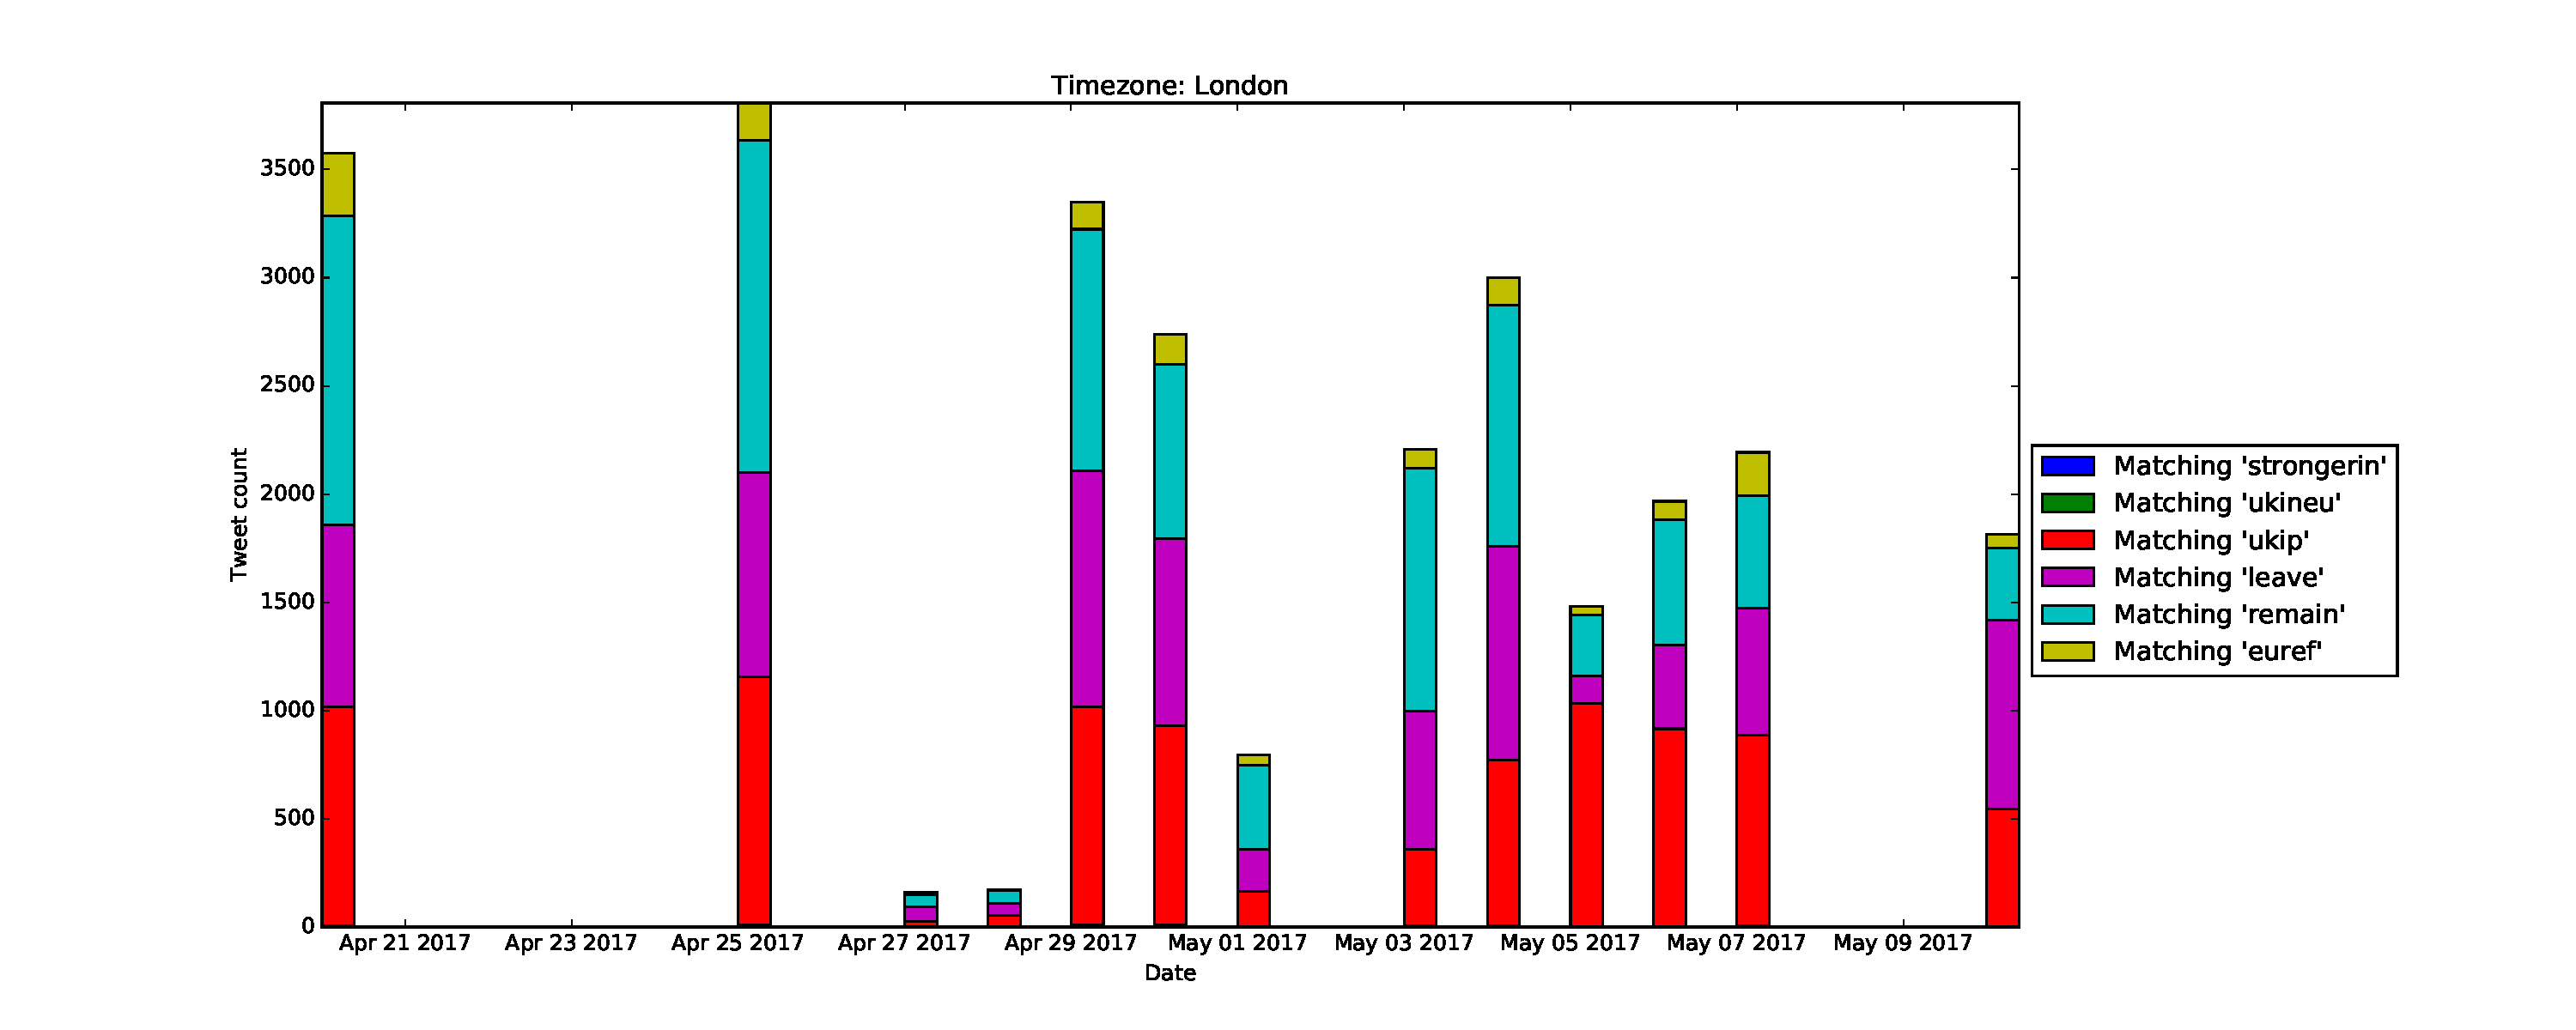
\includegraphics[width=1.1\linewidth]{img/frequency_stacked_London.pdf}
  \caption{We counted the appearances of certain keywords in the Tweets for each day in our data.
           Words like ``ukip'' are very present over the whole time window. We excluded the keyword ``brexit'',
           as it is included in almost every Tweet. See \cref{fig:freqlondon} for a larger version of the same plot.\label{fig:frequency-london}}
  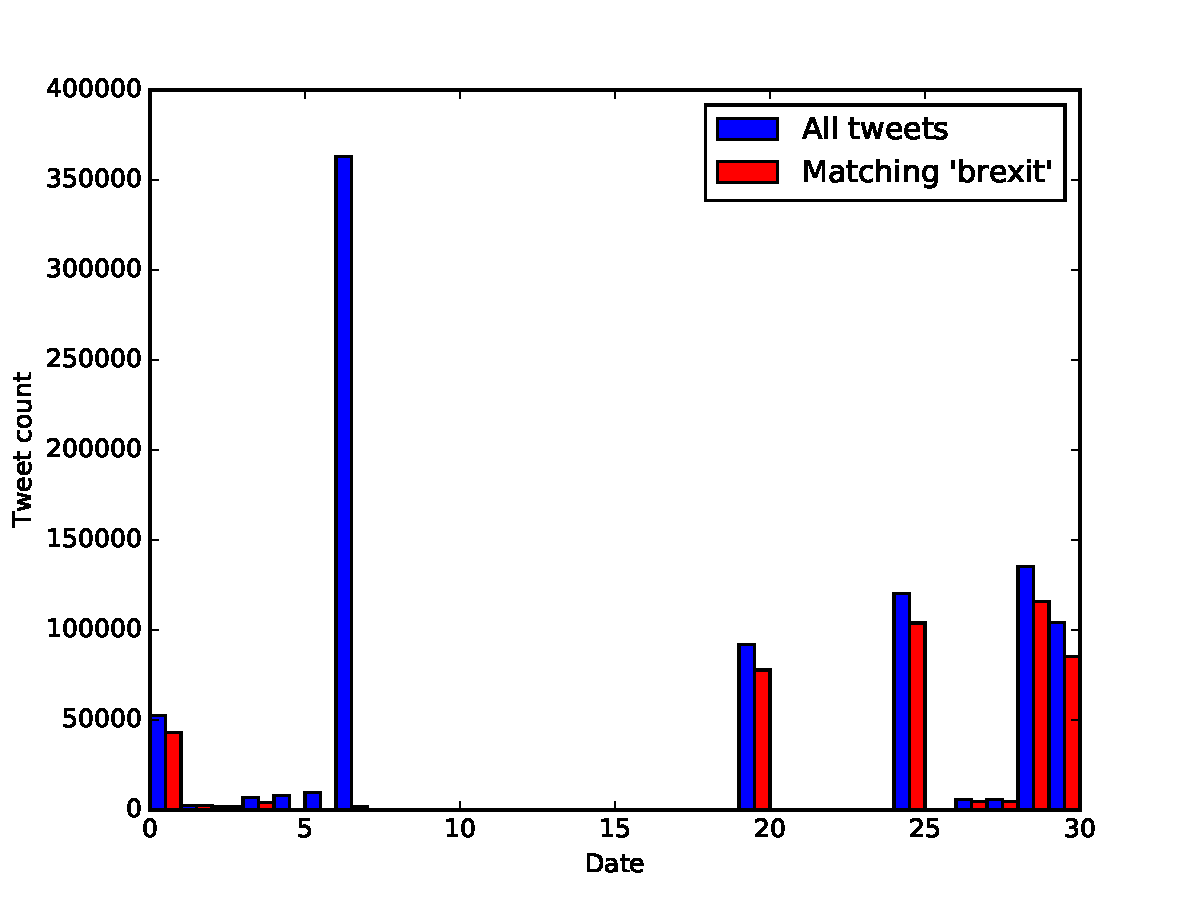
\includegraphics[width=1.1\linewidth]{img/frequency_brexit.pdf}
  \caption{Total activity of Brexit-related Tweets. As one can see almost all Tweets contain the keyword ``brexit'',
           thus it cannot be used to classify sentiments. However it is very useful to roughly filter for Tweets about
           the referendum.\label{fig:frequency-tot}}
\end{figure}
\clearpage

\section{Implementations}\label{sec:implementations}

\subsection{Language specifications}
We chose Python as our working language for several reasons.

Tweepy\cite{tweepy}, a Python library, grants easy access to the APIs. The sentiment analyser VADER is accessible as a Python library via github or the \texttt{nltk} module.
Pandas dataframes allow convenient manipulations of the data and Python's matplotlib can be used to visualise our results.

The gathered Twitter data was stored in a MySQL database.

\subsection{Data collection}

In order to get access to Twitter's APIs we created a Twitter account and used our user's access tokens for identification.

Twitter has four API classes --- two of which give us the Tweets, namely the REST APIs\cite{rest-apis} and the Streaming APIs\cite{streaming-apis}.
Latter gives low latency access to the global stream of Tweet data. It is suitable for long-term data mining, as it can simply be kept running in the background.
The REST APIs work on a request-response basis, meaning one has to send a request for certain keywords in a certain time and Twitter responds with the data. 

For our use the REST APIs had a distinct advantage: one has access to the data of the last seven days, and not only real-time.
As we had to crawl our data in a relatively short time we chose this access method over Streaming.
We had a Python script running on our server which sends requests for our keyword set on a regular basis and saves the formatted data to the MySQL database.
Our keywords are based on the hashtags proposed by Llewellyn and Cram\cite{llewllyn16}:
\begin{quote}
{\ttfamily
brexit, strongerin, euref, eureferendum, leaveeu, ukineu, voteleave, no2eu, 43brokenpromises, britainout
}
\end{quote}
We tried working with a larger set of keywords containing e.g. \texttt{\#go}, however the contribution of Tweets chosen by these new criteria 
turned out rather unsuitable. While we were gathering data of all languages - the hashtags used should stay the same in each language
and people may Tweet in english anyway - we only used Tweets of an \texttt{'en'} language. Checking foreign language Tweets in our database revealed that
they are mainly off-topic and not useful at all. Also, our analyser only works for english words, so a french Tweet with the keyword \texttt{brexit} doesn't help
us, as we cannot classify its sentiment.

Drawbacks of the REST APIs are the rate-limiting and the time-outs. 
We're only allowed to request a certain amount of data in a certain time, otherwise the interface throws an error.
Our script tried to take care of potential limits however sometimes the API threw an unexpected error and our program crashed.
We didn't always notice this immediately, which accounts for some days lacking in our plots.
In total we had about 1.3 million Tweets, 913 000 of which were marked as english. 
60-64\% of all our data were retweets: 767 000 in total and 588 000 in english.

As mentioned in the introduction we were provided with Tweets from 2016 by the COSS group at ETH. 
They were mining for a slightly different set of keywords. 
In \cref{fig:freqbrexit} we see the total count of Tweets per day and the count of Tweets containing the keyword \texttt{brexit}.
If the two bars are of similar height we expect almost all of Tweets to be relevant. 
In the data set from 2016 this is not the case and it could be that not all crawled Tweets are important. 
This, however, is not a severe problem as our sentiment analysis should categorise off-topic Tweets as ``other''.

\section{Results and Discussion}\label{sec:results}

Going back to \cref{fig:freqbrexit} we immediately notice two things: Large fluctuations aswell as a peak at the 29th of April 2017.
Days with apparently no Tweets originate from lacking measurements from us. 
The Tweet counts from 27th and 28th of April are suspiciously low and are most likely due to faulty or interrupted data mining.
On the 29th a Brexit-summit took place in Brussels\footnote{https://www.theguardian.com/politics/2017/apr/29/eu-\\leaders-set-to-take-tough-stance-in-special-brexit-summit
} % linebreak, otherwise doesn't fit in one line and we get an ugly indent
which caused a lot of attention.
Some other dates on which we would have expected a rise in attention were: February 20th and 21st, when prime minister James Cameron 
announced the date of the referendum\footnote{https://www.theguardian.com/politics/2016/feb/20/cameron-set-to-name-eu-referendum-date-after-cabinet-meeting}
and the day later former London major, Boris Johnson, joined the ``leave''-campaign\footnote{
https://www.theguardian.com/politics/2016/feb/21/boris-\\johnson-eu-referendum-campaign-for-brexit-david-cameron} aswell as April 15th, 
when the referendum campaign kicked off\footnote{https://www.theguardian.com/world/2016/apr/15/european-referendum-campaign-boris-johnson-alistair-darling}.
However in February the plots show no significant increase.

In \cref{fig:freqlondon,fig:freqmany} we broke the Tweet counts down to some of their constituents. 
The plot on the top shows our data from late April to beginning of May 2017 and the second row from February, April and May 2016.
We observe that the keyword \texttt{ukineu} vanishes very quickly and \texttt{ukip} rises in popularity.
In February 2016 keywords leaning towards ``leave'' are less prominent than in the following months.
In the bottom row we have again the data from 2017 but for different timezones.
The overall count distributions are similar for all of the four zones - with two main differences:
On April 25th the amount of Tweets in London and the US is significantly above the average. 
On the contrary, in Edinburgh the count on this day drops by 50\%.
In the US and Edinburgh we also discover a much lower prevalence of the keyword \texttt{leave}.
This result fits our expectations as the Scottish people favour staying in the EU\footnote{\label{bbc}http://www.bbc.com/news/uk-politics-36616028}.

\Cref{fig:totcount,fig:relcount} present the results from our sentiment analysis. 
We immediately notice that an overwhelming majority of the data has been classified ``stay''.
The category ``other'' accounts only for a vanishing percentage of all Tweets.
In the data from 2016 the composition of the categories does not change decidedly, whereas in 2017
we observe inconsitencies.
The Brexit vote took place on June 23rd 2016. We expected the fraction of ``stay''- and ``leave''-Tweets to change after this date,
as the vote was very controversial and the result came as a surprise to many people. 

A large amount of young people --- the demographic part of the population using Twitter more than any other and in favour of staying in the EU --- 
didn't cast their vote\footnoteref{bbc}.
Therefore a rise in ``stay''-Tweets would have been sensible in the end of June.
Unfortunately we have no access to data from this time and if we compare our pre-vote data with the post-vote data we cannot find a significant change.


%%
%% Appendix
%% 

\clearpage

\begin{appendix}

\begin{figure}[h]
  \plotone{img/Discr_ssix.png}
  \caption{Histogram of the sentiment values assigned by our ssix analyser. 
  The spectrum can be approximated as the sum of three Gaussian distributions. 
  The disciminants are set to the values where the Gaussians intersect.
  The three functions are $G(\mu,\sigma,\text{norm}) = G(-0.0131,4.47 \cdot 10^{-3}, 1.18), \
  G(-6.98 \cdot 10^{-4},1.33),3.50 \cdot 10^{-3}, 1.18)$ and  $G(0.0189,4.73 \cdot 10^{-3}, 0.83).$
  \label{fig:Discr-ssix}}
\end{figure}

\begin{figure}[h]
	\plotthree{img/leave_ssixKeywords.png}{img/stay_ssixKeywords.png}{img/other_ssixKeywords.png}
  	\caption{Distributions of our set of keywords in the training set Tweets with ``leave'', ``stay'' and ``other'' sentiment, respectively.
  Tweets containing a keyword with \texttt\# are only counted for the \texttt{\#keyword} piece of this pie chart and not again for the keyword without \texttt\#.
	\label{fig:category-ssixKeywords}}
\end{figure}
\begin{figure}
  \centering
  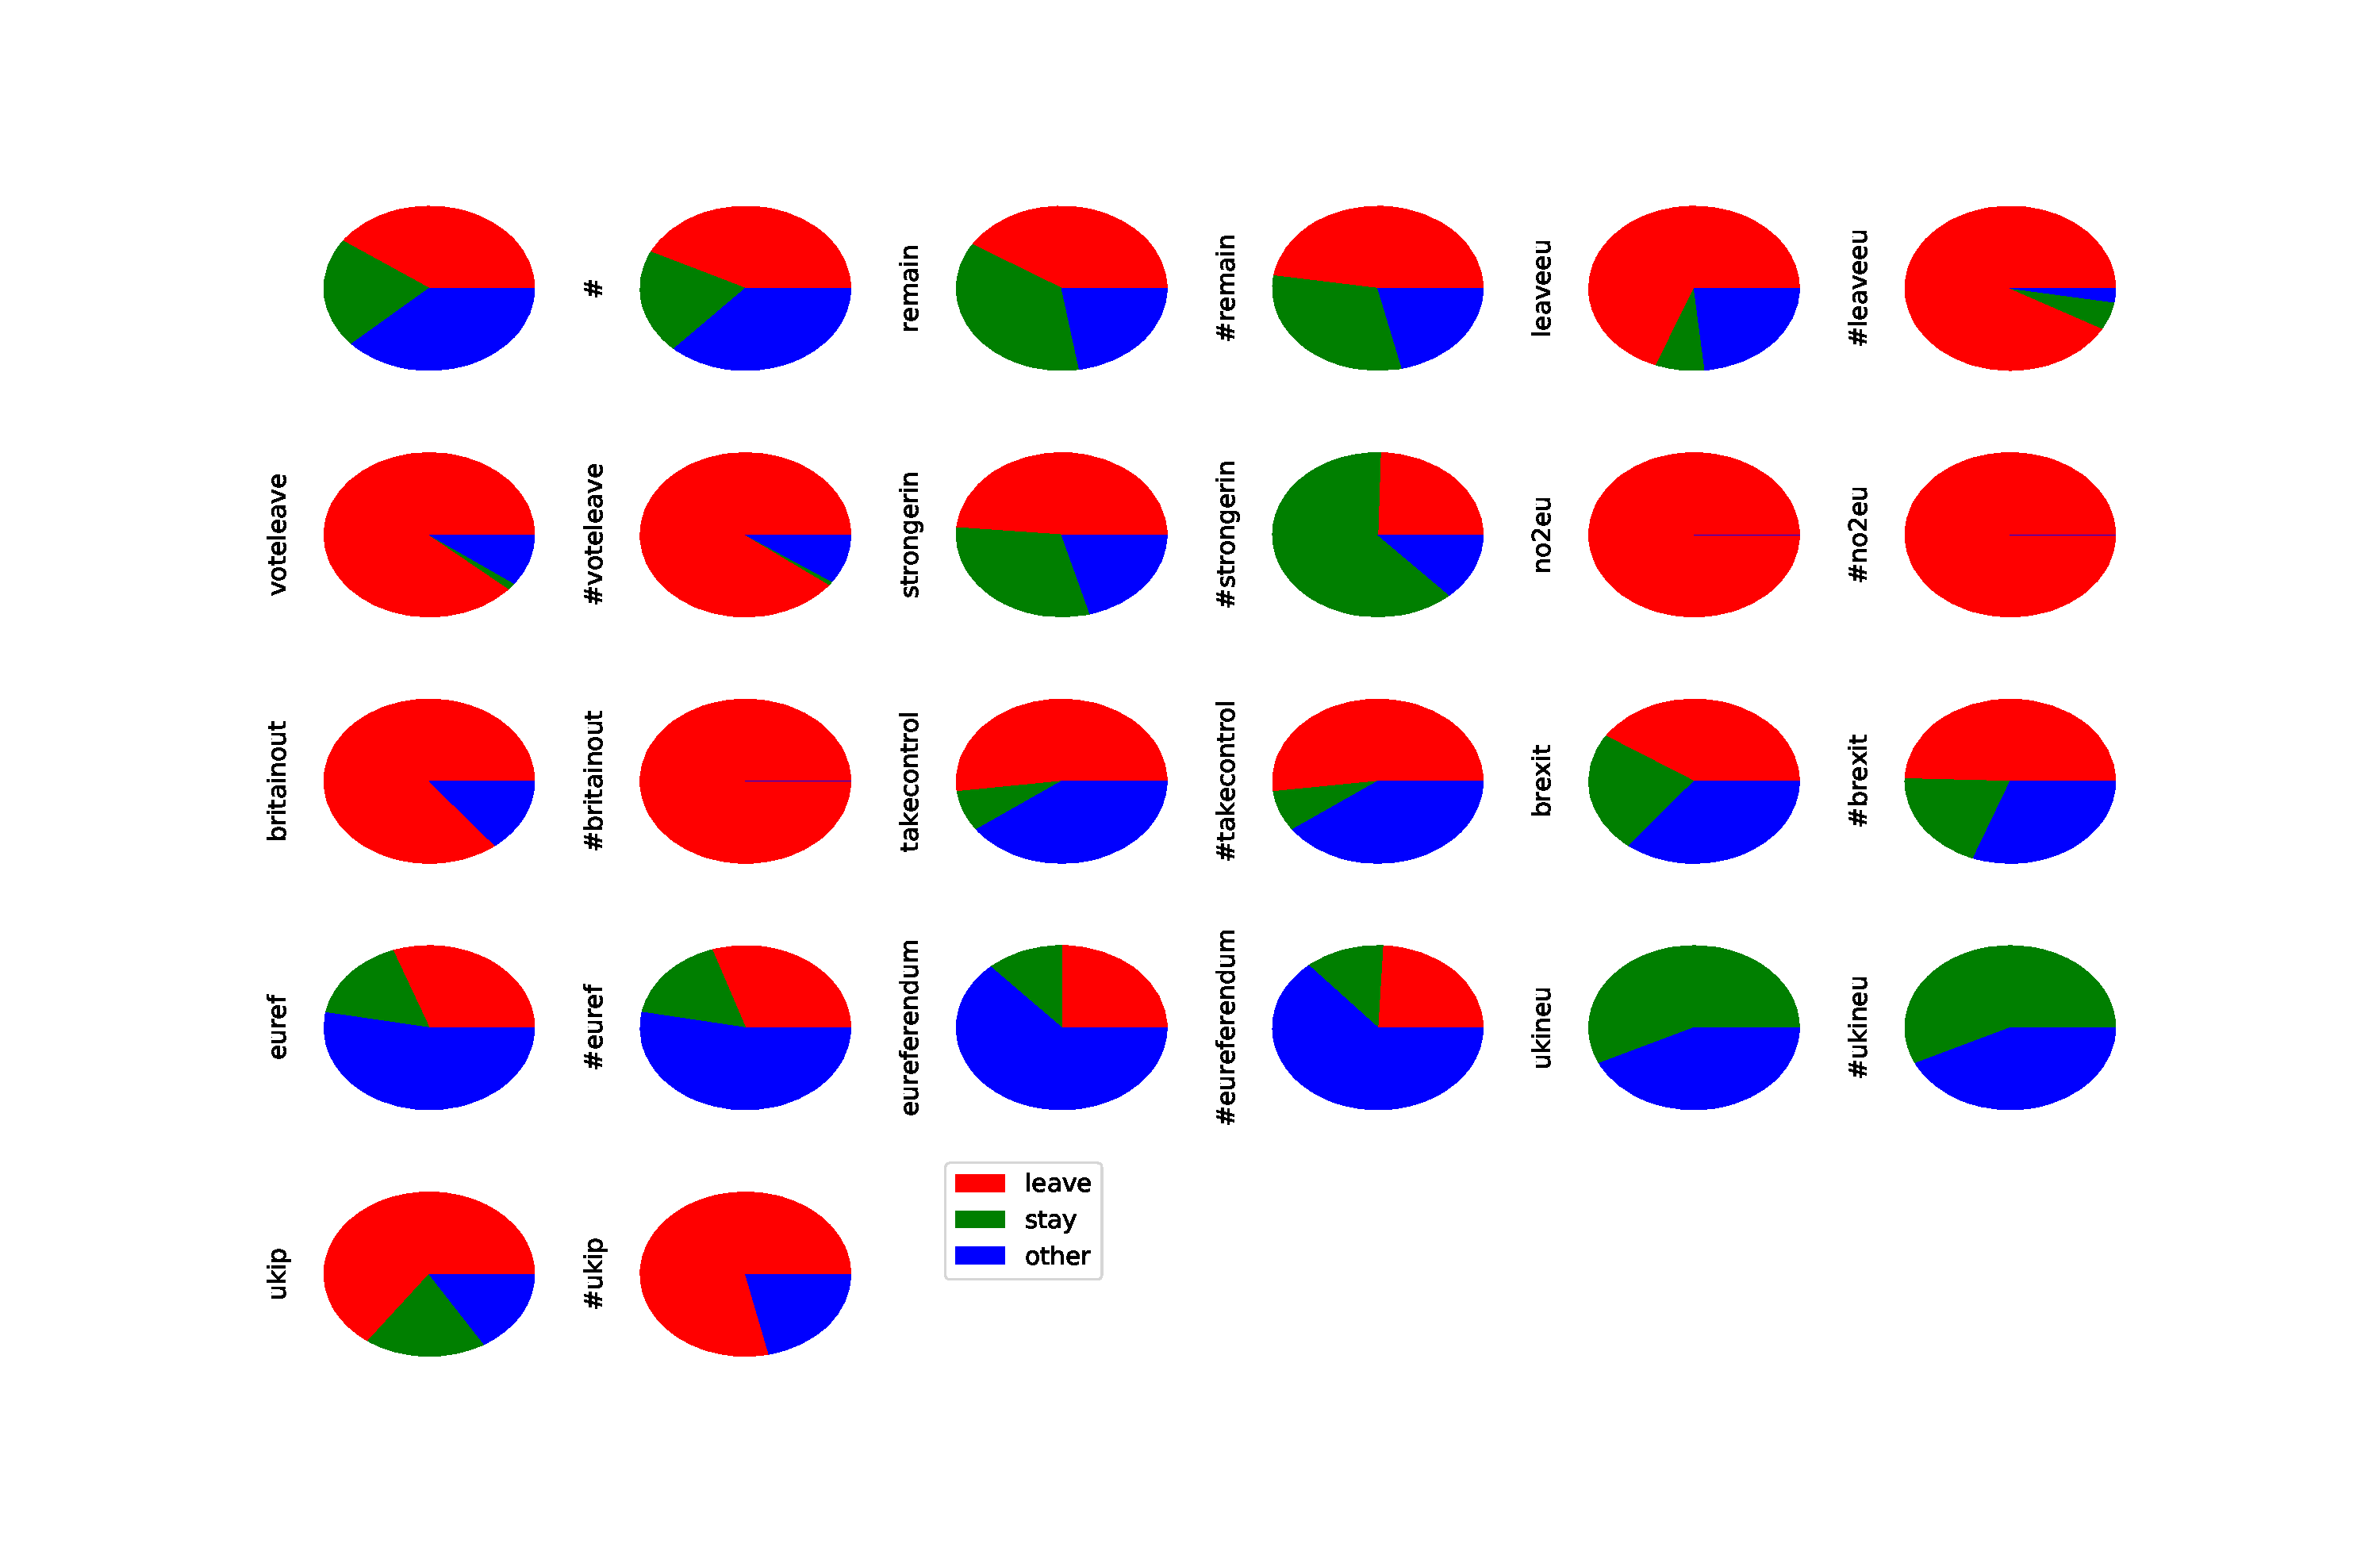
\includegraphics[width=0.6\textwidth]{img/keywords0.pdf}
  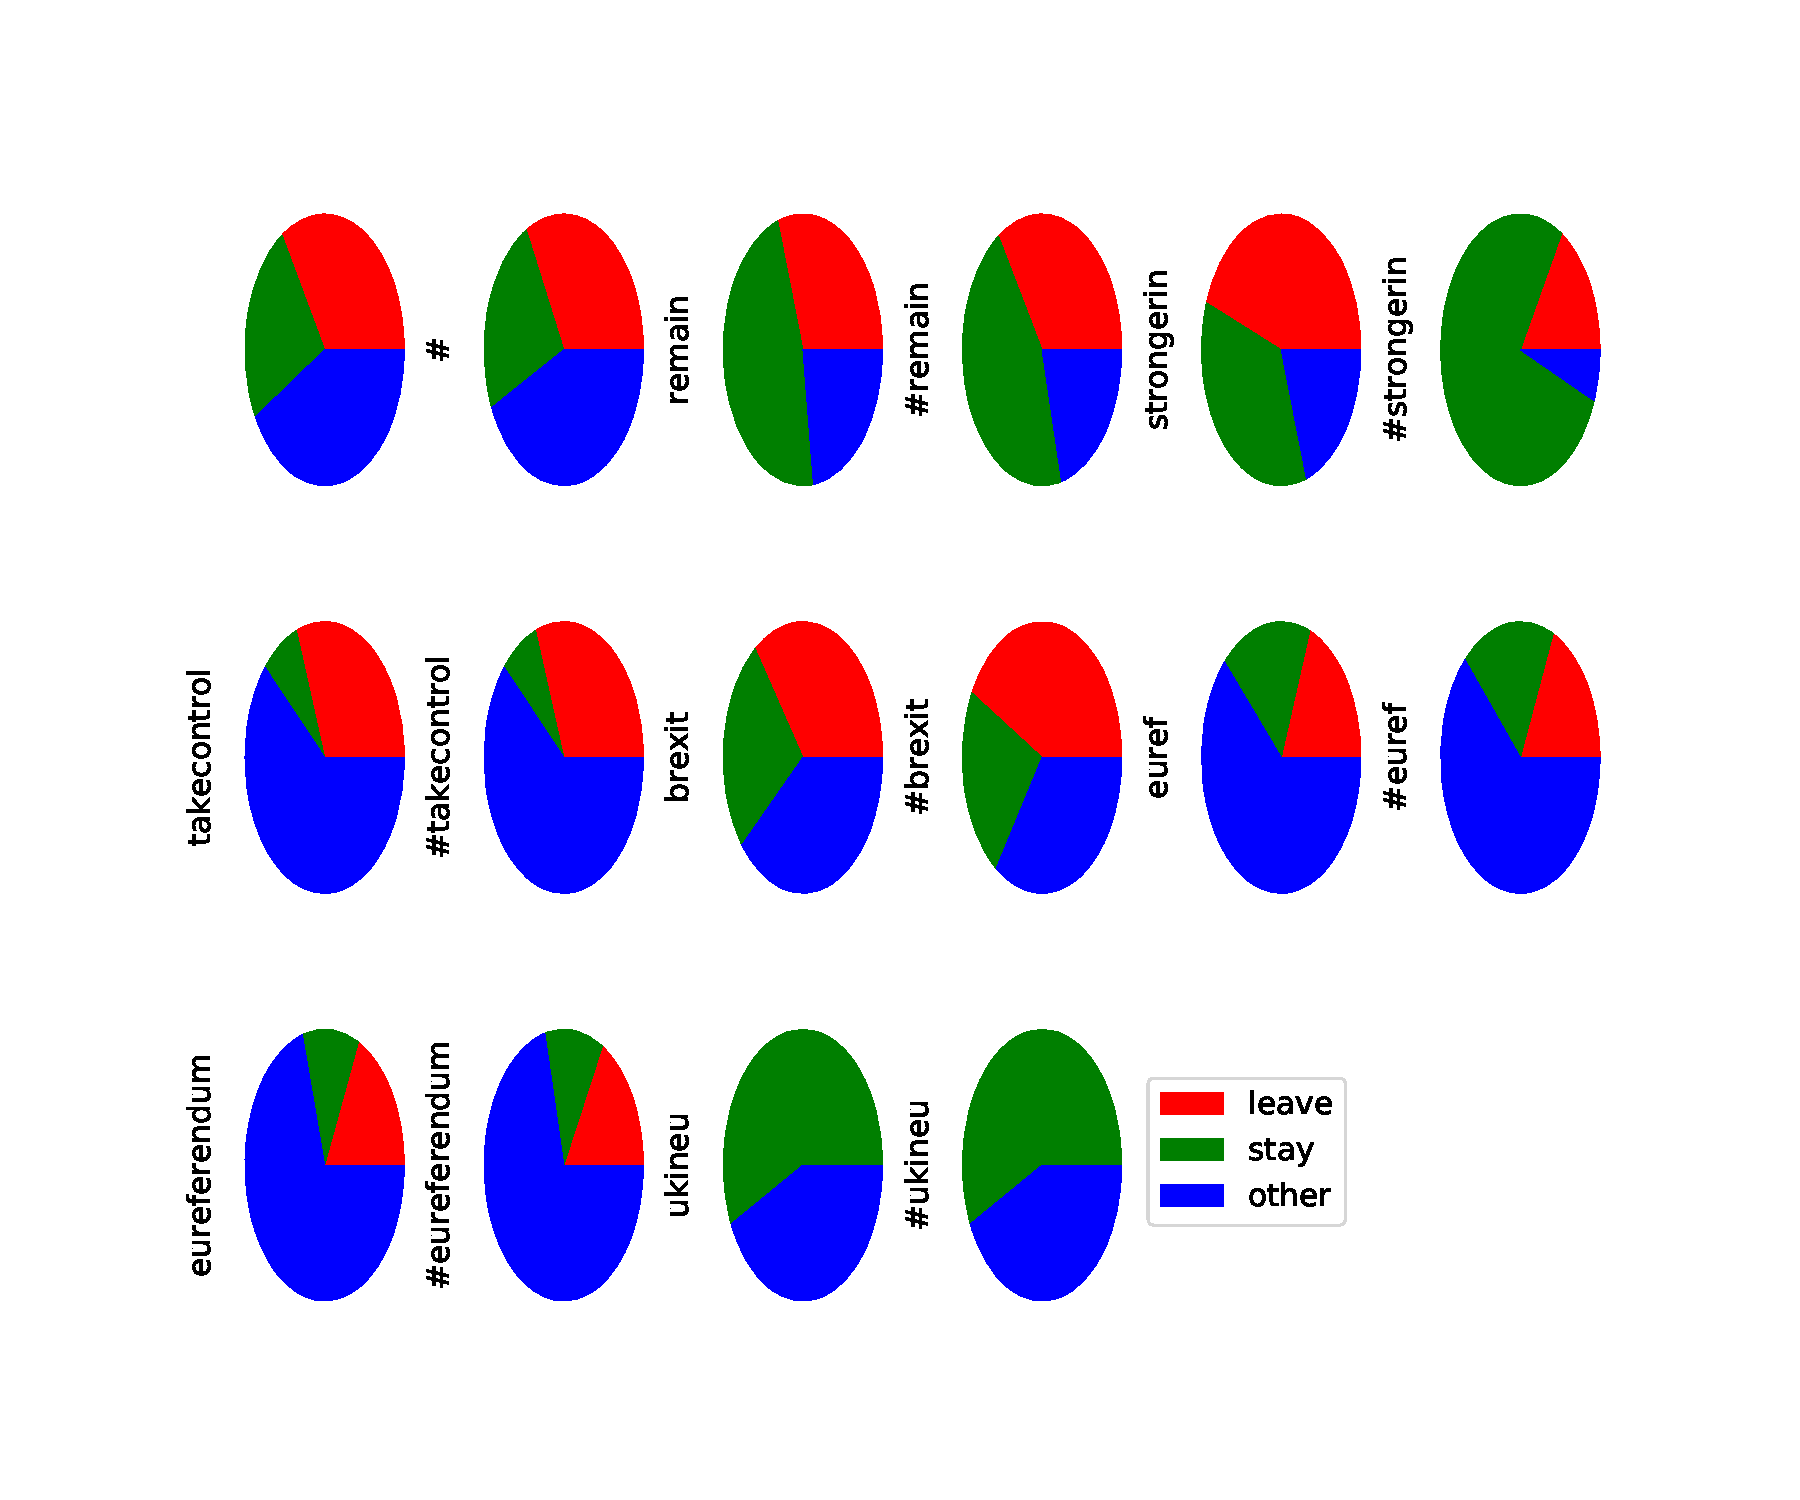
\includegraphics[height=0.3\textwidth, width=0.6\textwidth]{img/keywords1.pdf} \\
  \plottwo{img/keywords2.pdf}{img/keywords3.pdf}
  \caption{The first plot shows the sentiment distributions per keyword of the entire training set. 
  Obviously, the keys \texttt{leaveeu}, \texttt{\#leaveeu}, \texttt{voteleave}, \texttt{\#voteleave},
  \texttt{no2eu}, \texttt{\#no2eu}, \texttt{britainout}, \texttt{\#britainout}, \texttt{ukip} and \texttt{\#ukip}
  can be associated with the sentiment ``leave''.
  After removing all Tweets containing these classifiers we are left with the distributions in the second plot.
  Note, that the percentages have changed significantly, as Tweets can contain more than a single keyword.
  E.g.: If a Tweet contains \texttt{britainout, takecontrol} and \texttt{strongerin} it is already classified as ``leave'',
  and not considered anymore.
  In the second run we remove Tweets with the keywords: \texttt{euref, eureferendum} and \texttt{takecontrol}.
  Using a keyword as categoriser includes using the \texttt{\#}-version as the same categoriser.
  This goes on until the last plot, where no clear bias is observed. 
  For the remaining Tweets we will use our sentiment analysis.
  \label{fig:keywords}}
\end{figure}

\begin{figure} %ToDo: this one small?
  \centering
  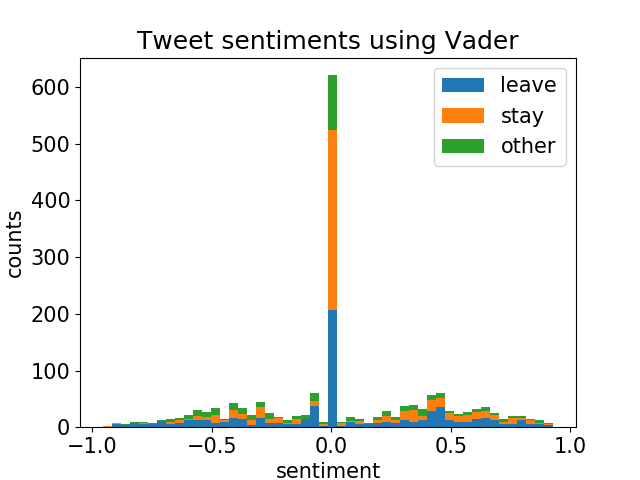
\includegraphics[width=0.5\linewidth]{img/vader_hist.png}
  \caption{Histogram of the sentiment values assigned by VADER.
  There is a high peak for zero sentiment. 
  The sentiments are almost equally distributed over the whole range. 
  \label{fig:vader-hist}}
\end{figure}
\begin{figure}
  \plotone{./img/frequency_brexit.pdf}
  \plotthree{./img/feb16/frequency_brexit}{./img/apr16/frequency_brexit}{./img/may16/frequency_brexit}
  \caption{The total amount of Tweets per day. Upper plot is created using our data from April to May 2017 and the ones below using the data provided by 
           the COSS group at ETH, which was using the Streaming APIs for data mining. 
           We see, that the Tweet count of the latter is much lower than the first, by about a factor 100.
           As we know that the Streaming APIs give access to ca. 1\% of the Tweets, we conclude that the REST APIs grant temporal access to the whole public data stream.
           \label{fig:freqbrexit}}
\end{figure}

\begin{figure}
  \plotone{./img/frequency_stacked_London.pdf}
  \plotthree{./img/feb16/frequency_stacked_London.pdf}{./img/apr16/frequency_stacked_London}{./img/may16/frequency_stacked_London}
  \caption{Keyword composition of the Tweets for the \texttt{user\_time\_zone} London, for April to May 2017 (upper plot) and certain dates in February, April 
  and May 2016 (lower plots).\label{fig:freqlondon}}
  \plotthree{./img/frequency_stacked_Dublin.pdf}{./img/frequency_stacked_Edinburgh.pdf}{./img/frequency_stacked_US.pdf}
  % No timezone Berlin available
  %\plotthree{./img/feb16/frequency_stacked_Berlin.pdf}{./img/apr16/frequency_stacked_Berlin}{./img/may16/frequency_stacked_Berlin}
  \caption{Keyword composition of the Tweets for the time zones Dublin, Edinburgh and US for late April and beginning of May 2017.\label{fig:freqmany}}
\end{figure}

\begin{figure}
  \plotone{./img/total_daycount_ls.pdf}
  \plotthree{./img/feb16/total_daycount_ls.pdf}{./img/apr16/total_daycount_ls.pdf}{./img/may16/total_daycount_ls.pdf}
  \caption{Day-for-day comparison of the number of Tweets pro-Brexit and contra, as categorised by our own sentiment analyser.
           On the top we see April and May 2017 and on the bottom selected dates in 2016.
  \label{fig:totcount}}
\end{figure}

\begin{figure}
  \plotone{./img/relative_daycount.pdf}
  \plotthree{./img/feb16/relative_daycount.pdf}{./img/apr16/relative_daycount.pdf}{./img/may16/relative_daycount.pdf}
  \caption{Relative day-for-day comparison of Tweets in favour of Brexit, against and without a strong sentiment, as categorised by our own sentiment analyser.
           On the top we see April and May 2017 and on the bottom selected dates in 2016.\label{fig:relcount}}
\end{figure}

\end{appendix}
%%
%% Bibliography
%%

\begin{thebibliography}{9}
  \bibitem[VADER()]{vader-paper} C.J. Hutto, Eric Gilbert (2014) VADER: A Parsimonious Rule-based Model for Sentiment Analysis of Social Media Text

  \bibitem[vaderSentiment()]{vader-code} VADER Sentiment Analysis, \\ 
    \url{https://github.com/cjhutto/vaderSentiment}

  \bibitem[SSIX GS()]{ssix} SSIX Brexit Gold Standard, \\
    \url{https://bitbucket.org/ssix-project/brexit-gold-standard}

  \bibitem[Tweepy()]{tweepy} Tweepy, \url{http://www.tweepy.org/}

  \bibitem[REST APIs()]{rest-apis} Twitter REST APIs, \\
    \url{https://dev.twitter.com/rest/public/search}

  \bibitem[Streaming APIs()]{streaming-apis} Twitter Streaming APIs, \\ 
    \url{https://dev.twitter.com/streaming/overview}

  \bibitem[Llewellyn (2016)]{llewllyn16} Clare Llewellyn, Laura Cram (2016) Brexit? Analyzing Opinion on the UK-EU Referendum within Twitter
\end{thebibliography}

\end{document}
